\documentclass{ximera}

\newcommand{\RR}{\mathbb R}
\renewcommand{\d}{\,d}
\newcommand{\dd}[2][]{\frac{d #1}{d #2}}
\renewcommand{\l}{\ell}
\newcommand{\ddx}{\frac{d}{dx}}
\newcommand{\dfn}{\textbf}
\newcommand{\eval}[1]{\bigg[ #1 \bigg]}


\author{Jason Miller}
\license{Creative Commons 3.0 By-NC}


\outcome{}


\begin{document}
\begin{exercise}
Use trig substitution to determine the integral.
\[
\int 50 x^{3} \sqrt{1-25x^{2}} \d x
\]

First we must determine the appropriate substitution. 

Since we have a $1-25x^{2}$ term, we should use $x=\answer{\frac{1}{5}\sin(\theta)}$. 

This means that $\d x= \answer{\frac{1}{5}\cos(\theta)} \d \theta$. 

\begin{exercise}
Using the trig identity $1-\sin^{2}(\theta)=\cos^{2}(\theta)$, we can rewrite $1-25x^{2}$ as $\answer{\cos^{2}(\theta)}$. 

Now we can express our original integral as a trigonometric integral in terms of the variable $\theta$. 

\[
\int  50 x^{3} \sqrt{1-25x^{2}} \d x= \int \answer{  \frac{2}{25} \sin^{3}(\theta) \cos^{2}(\theta)  } \d \theta\
\]

This is a trigonometric integral that can be evaluated easily by using the substitution $u = \answer{\cos(\theta)}$.  Carrying out the details, the antiderivative in terms of $\theta$ is: 

\[
\int \frac{2}{25} \sin^{3}(\theta) \cos^{2}(\theta)   \d \theta\ = \answer{ \frac{-2}{25}\left( \frac{\cos^{3}(\theta)}{3} -\frac{\cos^{5}(\theta)}{5} \right) + C}
\]
(Use $C$ for the constant of integration)


Now we really want the antiderivate in terms of $x$ since our functions was originally in terms of $x$. 

\begin{exercise}
Using the original substitution $x=\frac{1}{5}\sin(\theta)$, we draw the right triangle 

    \begin{image}
      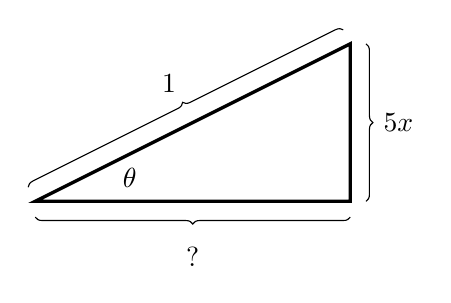
\begin{tikzpicture}
        \coordinate (C) at (0,2);
        \coordinate (D) at (4,2);
        \coordinate (E) at (4,4);
        \tkzMarkRightAngle(C,D,E)
        \tkzMarkAngle(D,C,E)
        \draw[decoration={brace,mirror,raise=.2cm},decorate,thin] (0,2)--(4,2);
        \draw[decoration={brace,mirror,raise=.2cm},decorate,thin] (4,2)--(4,4);
        \draw[decoration={brace,raise=.2cm},decorate,thin] (0,2)--(4,4);
        \draw[very thick] (D)--(E)--(C)--cycle;
        \node at (2,2-.7) {$?$}; %% adj
        \node[anchor=west] at (4+.3,3) {$5x$}; %% opp 
        \node at (2-.3,3+.5) {$1$}; %% hyp
        \node at (1.2,2.3) {$\theta$};
      \end{tikzpicture}
    \end{image}

Then using the Pythagorean Theorem we find that the
 length of the side adjacent to $\theta$ is $\answer{\sqrt{1-25x^{2}}}$. 

Using the triangle, we now convert each of the expressions in our antiderivative that was in terms of $\theta$ to be in terms of $x$:

\[
\cos(\theta)=\answer{\sqrt{1-25x^{2}}}
\]

\begin{exercise}
Hence the answer to our original integral is: 

\[
\int 50 x^{3} \sqrt{1-25x^{2}}  \d x= \answer{ \frac{-2}{25} \left( \frac{1}{3}(1-25x^{2})^{\frac{3}{2}} - \frac{1}{5}(1-25x^{2})^{\frac{5}{2}}\right) + C }
\]
(Use $C$ for the constant of integration)





\end{exercise}
\end{exercise}

\end{exercise}

\end{exercise}
\end{document}
